%===================================================================================
% Chapter: Proposed Solution
%===================================================================================
\Chapter{Propuesta de Solución}\label{chapter:proposed_solution}
\vspace{-0.3in}
Esta investigación busca poder expresar un corpus anotado a través de una ontología definida, generando un grafo de conocimiento como resultado. Otro de los objetivos claros, es poder hacer esto de forma automática mediante un algoritmo computacional.
%===================================================================================

\vspace{-0.1in}
\section{Analizador sintáctico}
\vspace{-0.1in}
Primeramente, es necesaria la creación de una herramienta capaz de fragmentar en objetos con significado computacional el contenido de los archivos de anotación escritos con el formato visto en la sección \ref{section:annotation_file_format}.

Dado que en el formato de archivo propuesto contiene una única relación anotada por línea y a su vez, las relaciones tienen su formato de escritura bien definido y sin ambigüedades, llevar a cabo la implementación de este analizador sintáctico es bastante sencillo. Esto puede hacerse a través de expresiones regulares, las cuales son ampliamente usadas y muchos de los lenguajes de programación modernos las incluyen como estructuras integradas.

\vspace{-0.1in}
\section{Modelo ontológico}
\vspace{-0.1in}
La ontología propuesta es de propósito general y basada en el modelo de anotación visto en la sección \ref{section:annotation_structure}. Esto posibilita la continuidad del proceso, partiendo desde documentos escritos en lenguaje natural, hasta la creación de una base de conocimiento a partir de ellos.

Una ontología $O=(C,~R,~A,~Top)$ se define mediante un conjunto no vacío de conceptos $C$, un conjunto de relaciones $R$, un conjunto de axiomas $A$ y $Top$ es el concepto con más alto nivel en la jerarquía. En esta investigación, la ontología propuesta es generada de forma automática, por tanto, las instancias pertenecientes a los conjuntos $C$ y $R$ son generadas de manera automática a medida que se procesa el corpus anotado. Dado que la ontología propuesta no tiene conocimiento previo del dominio, el conjunto $A$ es vacío. A la vez que $Top$ no se sabe a priori qué entidad o instancia de entidad es.

En contraste a definir las instancias de los conjuntos $C$ y $R$, son definidas las clases que serán usadas como base de creación de instancias que pertenecen al conjunto $C$ y las posibles relaciones entre estos, las cuales alimentarán al conjunto $R$ a medida que se va generando la ontología.

Todo concepto en la ontología pertenece a una de las tres clases siguientes: \textit{entidad simple}, \textit{entidad con atributo} o \textit{entidad compuesta}. El significado específico de estas clases, la creación de instancias a partir de ellas y las relaciones que pueden existir entre ellas son explicadas en las secciones siguientes.

\vspace{-0.1in}
\subsection{Clases en la ontología}
\vspace{-0.1in}
Los conceptos usados en la ontología propuesta en esta investigación pertenecen a una de las tres clases siguientes:

\vspace{-0.1in}
\begin{itemize}
	\item[•] Entidad simple: la más sencilla de las clases, no tiene ningún significado especial. En el modelo de la sección \ref{section:annotation_structure} representa un concepto sin haberle aplicado relaciones ni atributos. Cada concepto del modelo de anotación representa una entidad simple. Al ser creada una instancia, la propiedad \guillemot{\texttt{tipo de concepto}} adopta el valor del tipo de concepto específico en el corpus anotado de la palabra o frase correspondiente a la entidad.
	\item[•] Entidad con atributo: está compuesta por una \textit{entidad simple} y uno o más atributos de los mencionados en la sección \ref{section:annotation_structure}. Puede verse como el resultado de haber aplicado todos los atributos pertenecientes a un mismo concepto. Al ser creada una instancia, la propiedad \guillemot{\texttt{tipo de concepto}} adopta el valor del \guillemot{\texttt{tipo de concepto}} de la \textit{entidad simple} que le corresponde.
	\item[•] Entidad compuesta: es el resultado de aplicar las relaciones en el modelo de anotación explicado en la sección \ref{section:annotation_structure}. Está compuesta por la entidad correspondiente al origen y una o más entidades que son objetivos de dicha relación. Al ser creada una instancia, la propiedad \guillemot{\texttt{tipo de concepto}} adopta el valor del \guillemot{\texttt{tipo de concepto}} de la entidad origen que le corresponde.
\end{itemize}

\vspace{-0.1in}
Estas clases contienen, además, dos propiedades; una de ellas es la palabra o fragmento de texto en sí que representa la entidad y la otra es el tipo de concepto al que representan. Esta última propiedad se basa en los cuatro tipos de concepto existentes en el modelo de anotación explicado en la sección \ref{section:annotation_structure}, estos son: \textit{Concept}, \textit{Action}, \textit{Reference} y \textit{Predicate}.

No existen relaciones entre conceptos utilizados en el modelo de anotación y entidades debido a que cada concepto en el corpus anotado pasa a ser una instancia de entidad simple en la ontología. Por tanto, estas relaciones traerían consigo tener nodos inactivos o duplicados, dado que la información estaría duplicada en nodos de tipo concepto y nodos de tipo entidad simple, y además, las relaciones entre estos no aportarían conocimiento nuevo, en cambio, añadirían redundancia a la base de conocimiento.

\vspace{-0.2in}
\subsection{Relaciones en la ontología}
Los tipos de relaciones definidos en la ontología tienen una estrecha relación con los trece tipos de relación vistos en la sección \ref{section:relation_annotation}. Los actores pertenecientes a estas se describen en las secciones siguientes.

\vspace{-0.1in}
\subsubsection{Relación subject}
\vspace{-0.1in}
Puede tener cualquier instancia de entidad como origen y cualquiera como destino. La única restricción es que la entidad de origen debe tener \textit{Action} en la propiedad \guillemot{\texttt{tipo de concepto}}.

\vspace{-0.1in}
\subsubsection{Relación target}
\vspace{-0.1in}
Puede tener cualquier instancia de entidad como origen y cualquiera como destino. La única restricción es que la entidad de origen debe tener \textit{Action} en la propiedad \guillemot{\texttt{tipo de concepto}}.

\vspace{-0.2in}
\subsubsection{Relación domain}
Puede tener cualquier instancia de entidad como origen y cualquiera como destino. La única restricción es que la entidad de origen debe tener \textit{Predicate} en la propiedad \guillemot{\texttt{tipo de concepto}}.

\vspace{-0.1in}
\subsubsection{Relación argument}
\vspace{-0.1in}
Puede tener cualquier instancia de entidad como origen y cualquiera como destino. La única restricción es que la entidad de origen debe tener \textit{Predicate} en la propiedad \guillemot{\texttt{tipo de concepto}}.

\vspace{-0.1in}
\subsubsection{Relación is-a}
\vspace{-0.1in}
Puede tener cualquier instancia de entidad como origen y cualquiera como destino. Relación taxonómica que potencialmente da la posibilidad de descubrir de conocimiento.

\vspace{-0.1in}
\subsubsection{Relación part-of}
\vspace{-0.1in}
Puede tener cualquier instancia de entidad como origen y cualquiera como destino. Relación taxonómica que potencialmente da la posibilidad de descubrir de conocimiento.

\vspace{-0.1in}
\subsubsection{Relación same-as}
\vspace{-0.1in}
Puede tener cualquier instancia de entidad como origen y cualquiera como destino. Relación taxonómica que potencialmente da la posibilidad de descubrir de conocimiento.

\vspace{-0.1in}
\subsubsection{Relación has-property}
\vspace{-0.1in}
Puede tener cualquier instancia de entidad como origen y cualquiera como destino. Relación taxonómica que potencialmente da la posibilidad de descubrir de conocimiento.

\vspace{-0.1in}
\subsubsection{Relación causes}
\vspace{-0.1in}
Puede tener cualquier instancia de entidad como origen y cualquiera como destino. Relación que potencialmente da la posibilidad de descubrir de conocimiento.

\vspace{-0.1in}
\subsubsection{Relación entails}
\vspace{-0.1in}
Puede tener cualquier instancia de entidad como origen y cualquiera como destino. Relación que potencialmente da la posibilidad de descubrir de conocimiento.

\vspace{-0.1in}
\subsubsection{Relación in-time}
\vspace{-0.1in}
Puede tener cualquier instancia de entidad como origen y cualquiera como destino.

\vspace{-0.1in}
\subsubsection{Relación in-place}
\vspace{-0.1in}
Puede tener cualquier instancia de entidad como origen y cualquiera como destino.

\vspace{-0.1in}
\subsubsection{Relación in-context}
\vspace{-0.1in}
Puede tener cualquier instancia de entidad como origen y cualquiera como destino.

La relación directa entre dos instancias de entidades en la base de conocimiento implica la existencia de una relación directa entre ellos en el corpus anotado y viceversa. Por tanto, todo el conocimiento explícito descrito por el corpus será representado por relaciones entre instancias de entidades. Basado en esto, dado un camino $P$ de tamaño dos o más entre dos instancias de entidades $u$ y $v$ en este grafo y además, todas las aristas en $P$ son aristas que posibilitan el descubrimiento de conocimiento, entonces si no existe una arista directamente entre el nodo $u$ y el nodo $v$, el conocimiento inferido por el camino $P$ es válido e implícito en el corpus, por tanto, es conocimiento aprendido.

El proceso de creación de una base de conocimiento específica a partir de la definición de esta ontología es llevado a cabo de forma totalmente automática y no de la manera tradicional, con expertos en el dominio añadiendo relaciones entre clases una tras otra. A la interrogante de en qué orden se llevan a cabo estas relaciones y quiénes participan en ellas se le da respuesta en la próxima sección.

\section{Grafo de conocimiento}
\vspace{-0.1in}
Una vez que se haya analizado sintácticamente todo el corpus, se tendrá la información de las anotaciones en objetos computacionales y será más sencillo el trabajo con estos. En aras de evitar ambigüedades y concentrar el conocimiento para un mejor entendimiento de este y a la misma vez, poder facilitar la tarea de extraerlo de este grafo por un equipo de cómputo, el texto anotado es normalizado. Esto es llevado a cabo teniendo en cuenta las palabras que lo componen, y anotando en su lugar la palabra primitiva de esta. Por ejemplo, la palabra \guillemot{\texttt{sangramiento}} será anotada como \guillemot{\texttt{sangrar}} y la frase \guillemot{\texttt{glóbulos rojos}} como \guillemot{\texttt{glóbulo rojo}}.

Como se vio en la sección \ref{section:annotation_structure}, es necesario aclarar que hay que darle un orden a la creación de las instancias de las clases y las relaciones en este grafo, pues las propias anotaciones de texto y las relaciones tienen un orden implícito entre ellas. Por ejemplo, en la propia figura \ref{fig:annotation_example_composing_concepts}, se debe procesar primero el rol ejercido por \guillemot{\texttt{problemas}} y por \guillemot{\texttt{cumpla}} antes de poder procesar \guillemot{\texttt{impiden}}; de lo contrario, el conocimiento descrito por \guillemot{\texttt{impiden}} quedaría incompleto o mal representado.

\vspace{-0.1in}
\subsection{Orden topológico}
\vspace{-0.1in}
El orden establecido por el modelo de anotación visto en el capítulo \ref{chapter:annotation_model} es un orden topológico. Para ello se tiene en cuenta el siguiente orden:

\begin{enumerate}\label{enum:knowledge_graph_build_order}
	\vspace{-0.1in}
	\item Texto: son procesados primero los conceptos del corpus anotado, los cuales son convertidos a instancias de \textit{entidad simple}.
	\vspace{-0.1in}
	\item Atributos: luego son procesados aquellos conceptos que son modificados por atributos en el corpus anotado, los cuales son convertidos a instancias de \textit{entidad con atributo}, usando como base la \textit{entidad simple} correspondiente a dicho concepto.
	\vspace{-0.1in}
	\item Relaciones de acción, predicado y contextualización: luego se procesan estas relaciones, las cuales son representadas por instancias de \textit{entidad compuesta}. Además, para cada concepto que actúa en ellas, se busca su correspondiente instancia de entidad perteneciente al grafo de conocimiento.
	\vspace{-0.1in}
	\item Relaciones taxonómicas y de causa e implicación: por último son añadidas las relaciones que posibilitan el descubrimiento ímplicito en el corpus. Estas no representan nodos en el grafo, y de igual forma que en el paso anterior, para cada concepto que actúa en ellas, se busca su correspondiente instancia de entidad perteneciente al grafo de conocimiento.
\end{enumerate}

Una vez divididas las relaciones en estos tres grupos, estas son asociadas nuevamente, esta vez teniendo en cuenta la parte izquierda de cada una de ellas (\texttt{Arg1} en el archivo de anotación). Una instancia de clase es creada por cada una de estas agrupaciones resultantes, además, una instancia creada en un nivel más avanzado, teniendo en cuenta el orden visto anteriormente, representa una mayor cantidad de información y al mismo tiempo, información más específica respecto a su instancia asociada en niveles anteriores.

\subsection{Ejemplos de generación automática de ontologías}
A continuación se presentan dos ejemplos de la creación de una base de conocimiento a partir de un corpus anotado. En ambos casos, el corpus solo contiene un documento, y este está compuesto por una sola oración. La flecha que puede haber en algunas líneas de los documentos de ejemplo, significa que esta en el mismo es muy larga para ser mostrada en una única línea en este escrito y se continuará escribiendo debajo. En estos ejemplos, las palabras o frases no son normalizadas para un mejor entendimiento en lenguaje natural y además, porque hay varias formas, métodos y decisiones de cómo normalizar palabras o frases.

\subsubsection{Primer ejemplo}
En la figura \ref{fig:text_document1} puede verse el documento de texto de prueba empleado en el primer ejemplo. A su vez, en la figura \ref{fig:annotated_document1} se ve el documento anotado asociado a este. Como puede apreciarse, se siguieron los convenios establecidos en la sección \ref{section:annotation_conventions}. Por último, la base de conocimiento generada para este ejemplo puede verse en la figura \ref{fig:knowledge_graph1.3}.

\begin{annexample}
	[backgroundcolor=black!5]
	{4.9in}
	{fig:text_document1}
	{Ejemplo 1: documento \doublequote{\texttt{desmayo.txt}}}
	{Ejemplo 1: documento \doublequote{\texttt{desmayo.txt}}.}
	El desmayo (o síncope) es una pérdida temporal de la {\scriptsize $\hookrightarrow$}\\
	conciencia.
\end{annexample}

\begin{annexample}
	[backgroundcolor=cyan!13]
	{4.9in}
	{fig:annotated_document1}
	{Ejemplo 1: documento \doublequote{\texttt{desmayo.ann}}}
	{Ejemplo 1: documento \doublequote{\texttt{desmayo.ann}}.}
	\# Sentence 1: El desmayo (o síncope) es una pérdida {\scriptsize $\hookrightarrow$}\\
	temporal de la conciencia.\\
	\# Keyphrases\\
	T1\space\space Concept 3 10\space\space\space\space desmayo\\
	T2\space\space Concept 14 21\space\space\space síncope\\
	T3\space\space Action 30 37\space\space\space\space pérdida\\
	T4\space\space Concept 38 46\space\space\space temporal\\
	T5\space\space Concept 53 63\space\space\space conciencia\\
	\# Relations\\
	R1\space\space is-a Arg1:T1 Arg2:T3\\
	R2\space\space in-context Arg1:T3 Arg2:T4\\
	R3\space\space target Arg1:T3 Arg2:T5\\
	\textasteriskcentered\space\space\space same-as T1 T2
\end{annexample}

Siguiendo el orden topológico establecido \hyperref[enum:knowledge_graph_build_order]{anteriormente}, se puede ver en la figura \ref{fig:knowledge_graph1.1} el grafo de conocimiento resultante luego de realizado el punto $1$, donde cada concepto del corpus anotado es transformado en una instancia de entidad simple en la base de conocimiento.

\begin{figure}[H]
	\begin{center}
		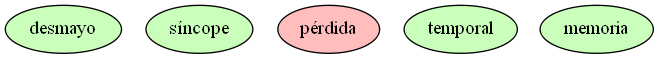
\includegraphics[width=4.5in]{graphics/knowledge_graph_example1_1.png}
		\caption[Ejemplo 1: grafo de conocimiento luego de realizado el punto 1]{Ejemplo 1: grafo de conocimiento luego de realizado el punto 1.}
		\label{fig:knowledge_graph1.1}
	\end{center}
\end{figure}

\vspace{-0.25in}
En el punto $2$ del orden topológico no puede hacerse nada en este corpus, pues no hay atributos, por tanto, el grafo de conocimiento quedará idéntico. Para el punto $3$ son usadas las relaciones \texttt{R2} y \texttt{R3}, resultando:

\vspace{-0.05in}
\begin{figure}[H]
	\begin{center}
		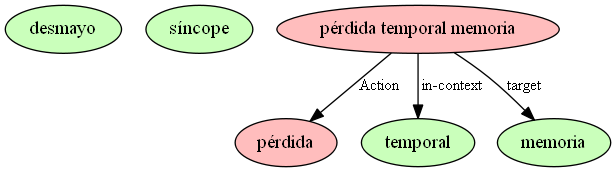
\includegraphics[width=4.7in]{graphics/knowledge_graph_example1_2.png}
		\caption[Ejemplo 1: grafo de conocimiento luego de realizado el punto 3]{Ejemplo 1: grafo de conocimiento luego de realizado el punto 3.}
		\label{fig:knowledge_graph1.2}
	\end{center}
\end{figure}

\vspace{-0.25in}
Para el punto $4$ son usadas las relaciones que potencialmente posibilitan el conocimiento ímplicito en el corpus. En este caso son: \texttt{R1} y \texttt{\textasteriskcentered}. Resultando:

\vspace{-0.05in}
\begin{figure}[H]
	\begin{center}
		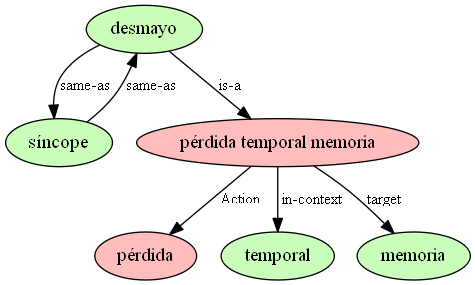
\includegraphics[width=3.6in]{graphics/knowledge_graph_example1_3.png}
		\caption[Ejemplo 1: grafo de conocimiento luego de realizado el punto 4]{Ejemplo 1: grafo de conocimiento luego de realizado el punto 4.}
		\label{fig:knowledge_graph1.3}
	\end{center}
\end{figure}

El ejemplo anterior es sencillo, pero aun así, puede descubrirse conocimiento implícito. Se infiere que \guillemot{\texttt{síncope} \textit{is-a} \texttt{pérdida temporal memoria}}.

\vspace{-0.1in}
\subsubsection{Segundo ejemplo}
\vspace{-0.1in}
En la figura \ref{fig:text_document2} puede verse el documento de texto de prueba empleado en el segundo ejemplo. A su vez, en la figura \ref{fig:annotated_document2} se ve el documento anotado asociado a este. Como puede apreciarse, en este documento también se siguieron los convenios establecidos en la sección \ref{section:annotation_conventions}. Por último, la base de conocimiento generada para este ejemplo puede verse en la figura \ref{fig:knowledge_graph2.4}.

\vspace{-0.1in}
\begin{annexample}
[backgroundcolor=black!5]
{\textwidth}
{fig:text_document2}
{Ejemplo 2: documento \doublequote{\texttt{higiene.txt}}}
{Ejemplo 2: documento \doublequote{\texttt{higiene.txt}}.}
	Las buenas prácticas de higiene, incluyendo lavarse las {\scriptsize $\hookrightarrow$}\\
	manos correctamente, pueden evitar infecciones.
\end{annexample}

\vspace{-0.2in}
\begin{annexample}
[backgroundcolor=cyan!13]
{\textwidth}
{fig:annotated_document2}
{Ejemplo 2: documento \doublequote{\texttt{higiene.ann}}}
{Ejemplo 2: documento \doublequote{\texttt{higiene.ann}}.}
	\# Sentence 1: Las buenas prácticas de higiene, incluyendo {\scriptsize $\hookrightarrow$}\\
	lavarse las manos correctamente, pueden evitar infecciones.\\
	\# Keyphrases\\
	T1\space\space Concept 4 10\space\space\space\space buenas\\
	T2\space\space Predicate 11 20 prácticas\\
	T3\space\space Concept 24 31\space\space\space higiene\\
	T4\space\space Action 44 51\space\space\space\space lavarse\\
	T5\space\space Concept 56 61\space\space\space manos\\
	T6\space\space Concept 62 75\space\space\space correctamente\\
	T7\space\space Action 84 90\space\space\space\space evitar\\
	T8\space\space Concept 91 102\space\space infecciones\\
	\# Relations\\
	R1\space\space in-context Arg1:T2 Arg2:T1\\
	R2\space\space domain Arg1:T2 Arg2:T3\\
	R3\space\space causes Arg1:T2 Arg2:T7\\
	R4\space\space is-a Arg1:T4 Arg2:T2\\
	R5\space\space target Arg1:T4 Arg2:T5\\
	R6\space\space in-context Arg1:T4 Arg2:T6\\
	R7\space\space target Arg1:T7 Arg2:T8\\
	\# Attributes\\
	A1\space\space Uncertain T7
\end{annexample}

Una vez más, siguiendo el orden establecido \hyperref[enum:knowledge_graph_build_order]{anteriormente}, se puede ver en la figura \ref{fig:knowledge_graph2.1} el grafo de conocimiento resultante luego de realizado el punto $1$, representando cada concepto del corpus anotado como una instancia de entidad simple.

\begin{figure}[H]
	\begin{center}
		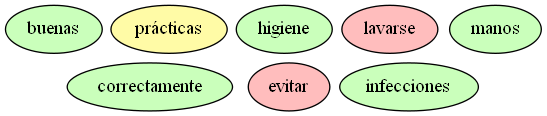
\includegraphics[width=4.2in]{graphics/knowledge_graph_example2_1.png}
		\caption[Ejemplo 2: grafo de conocimiento luego de realizado el punto 1]{Ejemplo 2: grafo de conocimiento luego de realizado el punto 1.}
		\label{fig:knowledge_graph2.1}
	\end{center}
\end{figure}

\vspace{-0.2in}
Dándole solución al punto $2$, los atributos del corpus anotado son representados como una instancia de entidad con atributo. Resultando:
\begin{figure}[H]
	\begin{center}
		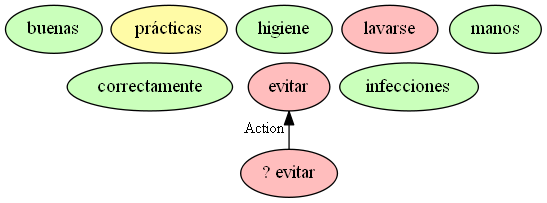
\includegraphics[width=4.2in]{graphics/knowledge_graph_example2_2.png}
		\caption[Ejemplo 2: grafo de conocimiento luego de realizado el punto 2]{Ejemplo 2: grafo de conocimiento luego de realizado el punto 2.}
		\label{fig:knowledge_graph2.2}
	\end{center}
\end{figure}

\vspace{-0.2in}
En aras de completar el punto $3$, las relaciones de acción, predicado y contextualización toman lugar. Resultando:
\begin{figure}[H]
	\begin{center}
		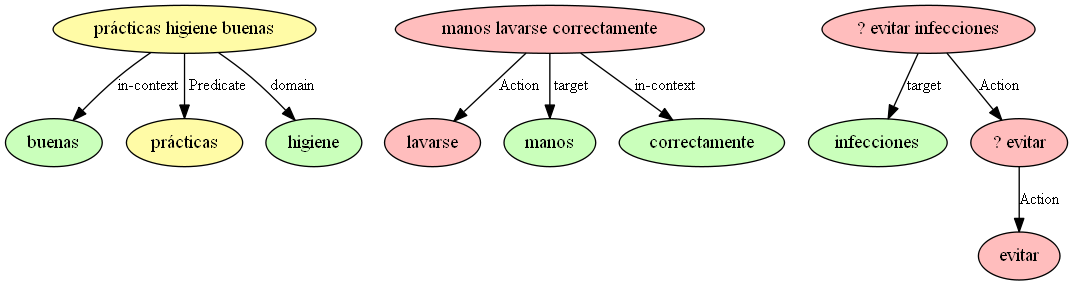
\includegraphics[width=\textwidth]{graphics/knowledge_graph_example2_3.png}
		\caption[Ejemplo 2: grafo de conocimiento luego de realizado el punto 3]{Ejemplo 2: grafo de conocimiento luego de realizado el punto 3.}
		\label{fig:knowledge_graph2.3}
	\end{center}
\end{figure}

Finalmente, al llevar a cabo el punto $4$, son agregadas las relaciones que posibilitan el descubrimiento de conocimiento implícito en el corpus. El grafo de conocimiento resultante de este ejemplo es:
\begin{figure}[H]
	\begin{center}
		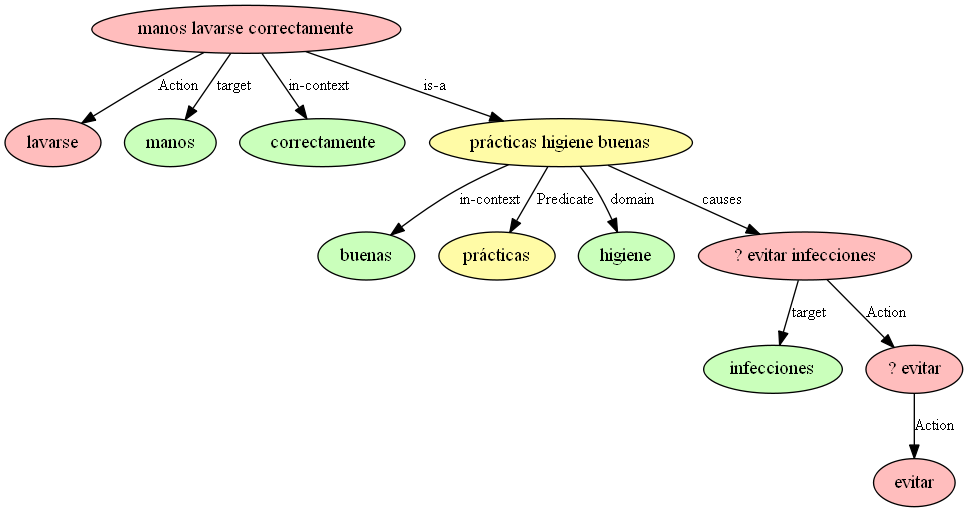
\includegraphics[width=\textwidth]{graphics/knowledge_graph_example2_4.png}
		\caption[Ejemplo 2: grafo de conocimiento luego de realizado el punto 4]{Ejemplo 2: grafo de conocimiento luego de realizado el punto 4.}
		\label{fig:knowledge_graph2.4}
	\end{center}
\end{figure}

Aunque el ejemplo anterior es sencillo, de igual forma que en el primer ejemplo, se puede descubrir conocimiento implícito. En esta ocasión se infiere que \guillemot{\texttt{manos lavarse correctamente} \textit{causes} \texttt{? evitar infecciones}}. Este conocimiento es traducido al lenguaje natural como \doublequote{lavarse las manos correctamente causa que puedan evitarse infecciones}.

Como pudo apreciarse en el ejemplo anterior, se optó por mostrar los atributos en el grafo a través de caracteres en vez de la palabra en sí. Son usados los siguientes caracteres:
\begin{itemize}
	\item[$\lnot$] negación
	\item[?] incertidumbre
	\item[$\downarrow$] disminución
	\item[$\uparrow$] énfasis
\end{itemize}

\subsection{Resumen del algoritmo}\label{section:ontology_construction}
Para llevar a cabo el punto $1$ en el orden previamente expuesto, se crea una \textit{entidad simple} por cada concepto existente en el documento de anotación. Esto sienta las bases para la posterior realización y correctitud del algoritmo expuesto en la sección anterior.

Para satisfacer lo propuesto en el punto $2$, cumplen un papel protagónico las entidades de los conceptos que tienen atributos asociados. En este punto, todas estas son del tipo \textit{entidad simple} y cada una de ellas se une con todos sus respectivos atributos, formando una \textit{entidad con atributo}.

En el paso $3$ tienen lugar algunas de las relaciones. Cada una de ellas conforma una \textit{entidad compuesta}. Esta nueva instancia se relaciona con los conceptos de las partes derecha de dichas relaciones, ahora representados en alguno de los tres tipos de clases de esta ontología, a través del tipo de relación. A la vez que se relaciona con la parte izquierda de estas por medio del tipo de entidad que sean.

El paso $4$ no crea instancias nuevas, solo establece la relación entre dos instancias creadas previamente en el grafo, aportando así conocimiento al mismo.

\section{Alineación de términos}
En el marco del ámbito social y mundial en que fue hecha esta investigación y por motivos principalmente de recursos, no pudo llevarse a cabo una investigación completa de este tema. En su lugar, se realizó un enfoque básico usando lematización y alineación de términos. Esto se logra por medio de la normalización de palabras o frases usadas como conceptos en el corpus anotado, una vez vayan a ser representados en la base de conocimiento. Además, se ofrecen estadísticas y resultados en este acercamiento al problema.

Con el paso del tiempo, la resolución de correferencias pasó de estar plenamente involucrado con este estudio a ser una recomendación para el futuro. Este problema es un primer acercamiento que mejorará la calidad y cantidad de conocimiento implícito descubierto, a la vez de mejorar los resultados alcanzados en esta investigación. De esta manera se dejan abiertas las puertas para la continuación y mejora de lo que aquí se presenta.